\documentclass{report}

\input{../../LatexTemp/preamble}
\input{../../LatexTemp/macros}
\input{../../LatexTemp/letterfonts}

 \title{\Huge{Analisi (M2)}\\Appunti}
\author{\huge{Alex Bastianini}}
\date{}

\setlength{\parindent}{0pt}
\usepackage{graphicx}
\usepackage{pgfplots}
\pgfplotsset{
    integral segments/.code={\pgfmathsetmacro\integralsegments{#1}},
    integral segments=3,
    integral/.style args={#1:#2}{
        ybar interval,
        domain=#1+((#2-#1)/\integralsegments)/2:#2+((#2-#1)/\integralsegments)/2,
        samples=\integralsegments+1,
        x filter/.code=\pgfmathparse{\pgfmathresult-((#2-#1)/\integralsegments)/2}
    }
}

\begin{document}
\maketitle
\newpage% or \cleardoublepage
% \pdfbookmark[<level>]{<title>}{<dest>}
\pdfbookmark[section]{\contentsname}{toc}
\tableofcontents
\pagebreak

\chapter{Introduzione agli appunti}
Questo e' un \textbf{test} per vedere come viene fuori un paragrafo di testo normale. Il testo sembra troppo piccolo pero.
\section{Le varie parti degli appunti}
Diversi box colorati per indicare diverse parti degli appunti:
\dfn{Definizione}{}
\thm{Teorema}{}
\pf{Dimostrazione}{}
\cor{Corollario}{}
\nt{Una roba importante}

\chapter{Integrali}
\section{Motivazioni}
Motivazioni:
\begin{itemize}
\item Calcolo di aree di figure curvilinee
\item Lunghezze di curve (non lo faremo)
\end{itemize}
Le nostre figure curvilinee sono sottografici di funzioni.
\section{Area sottesa a una curva}
\dfn{Area sottesa}{
  Data $f:[a,b] \to \mathbb{R}$
  \[
    A = \{(x,y) \in \mathbb{R}^2 | x \in [a,b]. 0 \leq y \leq f(x)\}
  \]
  
}
\subsection{Costruzione integrale di Riemann}
Speziamo un intervallo [a,b] in $n\in \mathbb{N}$ sottointervalli uguali. L'ampiezza di ciuascun intervallo e' di $\frac{b-a}{n}$. 
\begin{itemize}
\item $x_0 = a$
\item $x_1 = a + \frac{b-a}{n}$
\item $x_n = b$
\end{itemize}
In ogni intervallo fisso un punto arbirario $\epsilon_n$ 
\dfn{Somma di Riemann associata a una scomposizione}{
  Data una funzione $f:[a,b]\to\mathbb{R}$, fatta la costruzione precedente (spezzettamento), $\forall n \in \mathbb{N}$ la somma di Riemann n-esima di f e' il numero seguente:
  \[
  S_n = \sum_{k=1}^{n} f(\epsilon_k)(x_k - x_{k-1})
  \]
  
}
\begin{align}
  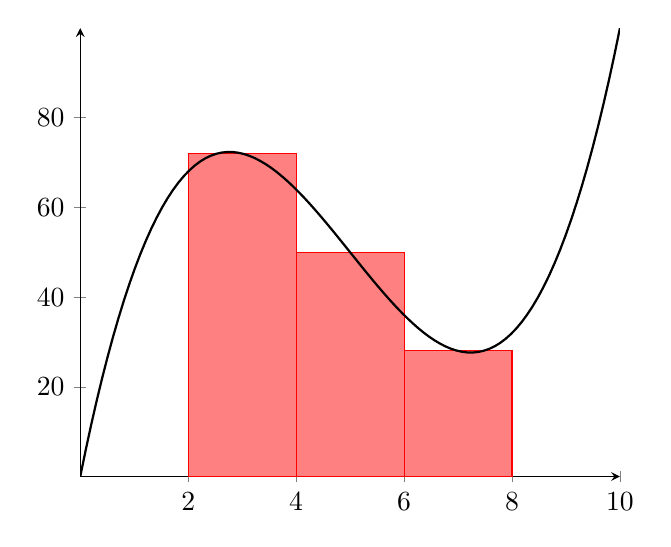
\begin{tikzpicture}[/pgf/declare function={f=-15*(x-5)+(x-5)^3+50;}]
    \begin{axis}[
        domain=0:10,
        samples=100,
        axis lines=middle
    ]
    \addplot [
        red,
        fill=red!50,
        integral=2:8
    ] {f};
    \addplot [thick] {f};
    \end{axis}
  \end{tikzpicture}
\end{align}
\begin{align*}
  \text{Esempio di somma di Riemann di una funzione $f:[2,8]\to\mathbb{R}$ con n=3:}
\end{align*}
\thm{Integrabilita' delle funzioni continue}{
  Sia $f:[a,b]\to\mathbb{R}$ continua. Sia $(S_n)$ la successione delle somme di Riemann, allora:
  \[
    \lim_{n\to +\infty} S_n = l \in \mathbb{R}
  \]
  E non dipende da quale $\epsilon_n$ scegliamo per ogni segmento.
}
\dfn{Integrale}{
  \[
    \int_{a}^{b} f(x)dx = \lim_{n\to+\infty} S_n
  \]
  La x e' una variabile \textbf{muta}. 
}
\nt{
\begin{itemize}
  \item Se $\forall x \in [a,b]. f(x) \geq 0$, allora $\int_a^b f$ = Area del sottografico.
  \item $\int_a^a f = 0$ (poiche $\forall n \in \mathbb{N}. S_n = 0$)
  \item $ f(x) = k (\text{funzione costante}) \implies \int_{a}^{b}f = (b-a)k (\text{Area del rettangolo}) $
\end{itemize}
}
\subsection{Proprieta' dell'integrale}
\subsubsection{Linearita'}
Se abbiamo due funzioni f, g continue su [a,b], $A, \mu \in \mathbb{R}$
\[
  \int^b_a (Af(x)+\mu g(x))dx = A\int^b_a f(x)dx + \mu\int^b_a g(x)dx
\]
\subsubsection{Additivita}
Data $f:[a,b]\to\mathbb{R}$ continua, dato $c \in [a,b]$, vale: \label{HA}
\[
\int^b_a f = \int^c_a f + \int^b_c f
\]
\nt{
Convenzione su integrali con estremi "rovesciati":\\
Dato $f:[a,b]\to\mathbb{R}$
\[
\int^b_a f = -\int^a_b f
\]
}
In questo modo possiamo generalizzare la proprieta' addittiva togliendo dall' ipotesi la restrizione sul valore di c.
\subsubsection{Monotonia}
Se $f:[a,b]\to\mathbb{R}$ e $\forall x \in [a,b]. f(x) \geq 0$, allora:
\[
\int^b_a f \geq 0 
\]
\subsection{Media Integrale}

\textbf{Premessa 1}\\
\thm{Valori intermedi}{
  Sia $f:[a,b]\to\mathbb{R}$ continua, $x_1, x_2, \in [a,b]. f(x_1) \leq f(x_2)$, allora:
  \[
    \forall y \in [f(x_1), f(x_2)].\exists c \in [x1, x2].f(c)=y
  \]
  
}
\textbf{Premessa 2}\\
\thm{Weierstrass}{
  Sia $f:[a,b]\to\mathbb{R}$ continua:
  \[
    \exists x_1, x_2 \in [a,b].\forall x \in [a,b]. f(x_1) \leq f(x) \leq f(x_2)
  \]
}
\begin{figure}[h!]
    \centering
    \includegraphics[width=50mm]{img/1200px-Extreme_Value_Theorem.svg.png}
    \caption{Esempio di Weierstrass}
  \end{figure}

\thm{Media integrale}{
  Sia $f:[a,b]\to\mathbb{R}$ continua, allora:
  \[
    \exists c \in [a,b]. \frac{1}{b-a}\int^b_a f(x)dx = f(c)
  \]      
}

\begin{figure}[h!]
  \centering
  \includegraphics[width=100mm]{img/2024-02-23-16-46-38.png}
\end{figure}

Quindi esiste un punto c in [a,b] t.c. il rettangolo che ha come base b-a e come altezza f(c) ha la stessa area dell'integrale di f da a a b.\\

\pf{Dimostrazione della media integrale}{
  Sia f continua su [a,b]. Per Weierstrass abbiamo che $\exists x_1, x_2 \in [a,b].\forall x \in [a,b].f(x_1) \leq f(x) \leq f(x_2)$. Per la proprieta' di monotonia risulta $\int^b_a f(x_1)dx \leq \int^b_a f(x)dx \leq \int^b_a f(x_2)dx$, ovvero $f(x_1) \leq \frac{1}{b-a}\int^b_a f(x)dx \leq f(x_2)$. Quindi per il teorema dei valori intermedi $\exists c \in [a,b].f(c)=\frac{1}{b-a}\int^b_a f(x)dx$.
}

\nt{
  La continuita' di f e' \textbf{necessaria}. Ex:
  \[
    f:[-1,1] \to \mathbb{R}, f(x) = x \implies \frac{1}{2} \int_{-1}^{1}xdx = 0 = f(0) (c=0)
  \]
 \begin{align*} 
    \begin{tikzpicture}
      \draw[->] (-1.5,0)--(1.5,0) node[below] {$ x $};
      \draw[->] (0,-1.5)--(0,1.5) node[left] {$ y $};
      \draw[domain=-1:1] plot (\x, \x);
      \draw[dashed] (1,0)--(1,1) (0.7, 0.3) node{$ A_1 $};
      \draw[dashed] (-1,0)--(-1,-1) (-0.7, -0.3) node{$ A_2 $};
      \draw (1.5, 1.5) node{$ A_1 = -A_2 $};
    \end{tikzpicture}
 \end{align*}
  Se considerassi $ g:[-1,1] \to \mathbb{R}$
  \[
    g(x) = \begin{cases}
    x & x \neq 0\\
    2 & x = 0
    \end{cases}
  \]
  Si dimostra che g e' intagarbile, e che vale
  \[
    \int_{-1}^{1}g(x)dx = 0
  \]
  Pero' non esiste $ c \in [-1,1] $ tale che g(c) = 0, quindi non soddisfa la media integrale.
}

\section{Primitive di una funzione}
\dfn{Primitiva di f}{
  Sia $ f: A \to \mathbb{R}, A \subseteq \mathbb{R} $\\
  Una funcione $ F: A \to \mathbb{R} $ si dice primitiva di f su A se vale
  \[
    \forall x \in A. F'(x) = f(x)
  \]
}
\ex{Primitiva}{
  $ f:\mathbb{R}\to \mathbb{R} $, $f(x) = \cos x \implies F(x) = sin x$ e' una primitiva di f su $ \mathbb{R} $. Infatti $\forall x. \frac{d}{dx}sinx = cosx $
}
\nt{
  $ \forall k \in \mathbb{R}\text{, la funzione }G(x) = sin(x)+k $ e' anchessa primitiva di $ f $. Quindi se $ F $ e' primitiva di $ f $ su A allora ci sono infinite primitive di $ f $ su A (una per ogni $ k \in \mathbb{R} $).\\
}
Domanda: sono tutte le possibili primitive?
\mprop{Caratterizzazione delle primitive di una funzione su un intervallo}{
  Sia $ f:]a,b[\to\mathbb{R}$. Siano $F:]a,b[\to\mathbb{R}\text{ e }G:]a,b[\to\mathbb{R}$ due primitive di $ f $ su $ ]a,b[ $.\\
  Allora $ \exists k \in \mathbb{R} $ tale che:
  \[
    \forall x \in ]a,b[. G(x)=F(x)+k
  \]
  Ovvero $ F $ e $ G $ "differiscono per una costante".
}
\pf{Dimostrazione}{
  Considero $ H:]a,b[\to\mathbb{R}, H(x)=G(x)-F(x) $. Sappiamo che F'(x)=f(x) e G'(x)=f(x) (def. primitiva).
  $ \frac{d}{dx}H(x) = \frac{d}{dx}G(x)-\frac{d}{dx}F(x) = f(x)-f(x) = 0 $. Dunque $ H $ ha derivata nulla su $ ]a,b[ $, quindi (per coroll. Lagrange) $ H $ e' costante.
}

\section{Funzioni integrali}
D'ora in poi $ A = ]a,b[ $.
\dfn{Funzione Integrale}{
  Sia $ f:A\to\mathbb{R} $ continua.\\
  Sia $ c\in A $. Introduco $ I_c:A\to\mathbb{R} $:
  \[
    I_c(x) = \int_{c}^{x}f(t)dt
  \]
  Nota: $ I_c $ e' ben definita essendo f continua.
}
\nt{
  \begin{enumerate}
    \item $ f:A\to\mathbb{R}, c\in A, I_c(x) = \int_{c}^{x}f \implies I_c(c)=\int_{c}^{c}f(t)dt = 0 $.
    \item Dati $ c,c' \in A, f:A\to\mathbb{R} \implies I_c(x)-I_{c'}(x) $ = costante. Infatti:
      \[
        I_c(x) - I_{c'}(x) = \int_{c}^{x}f - \int_{c'}^{x}f = \int_{c}^{x}f + \int_{x}^{c'}f = \int_{c}^{c'}f(t)dt = k
      \]
  \end{enumerate}
}
\subsection{Teoremi fondamentali del calcolo integrale}
\thm{Fondamentale del calcolo sulla derivata della funzione integrale}{
  Sia $ f:A\to\mathbb{R} $ continua, $ c \in A $. Sia $ I_c $ la funzione integrale, allora:
  \[
    I_c \text{ e' derivabile in ogni punto } x \in A \text{ e } I_c'(x) = f(x)
  \]
  Cioe' $ \frac{d}{dx}\int_{c}^{x}f(t)dt = f(x), \forall x \in A $, quindi $ I_c $ e' \textbf{primitiva} di $ f(x) $.
}
Una possibile interpretazione di questo teorema e' quello della derivata dell'area sottesa che e' uguale alla funzione stessa, ovvero:
\[
  \forall x. f(x) \geq 0 \implies \frac{d}{dx} \text{Area} = f(x)
\]
$ A = [-2,2], f(x)=\frac{x^2}{5} + 1 $:\\
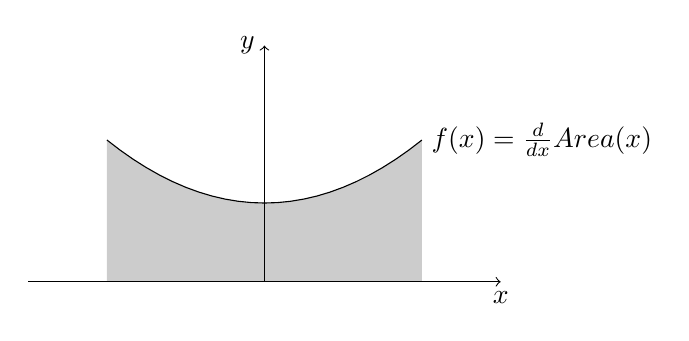
\begin{tikzpicture}
  \fill[gray!40, domain=-2:2, variable=\x]
   (-2,0)
   -- plot (\x, \x*\x/5 + 1)    
   -- (2,0)
   -- cycle;
   \draw[domain=-2:2] plot (\x, {(\x*\x/5 + 1)}) node[right]{$ f(x) = \frac{d}{dx}Area(x) $};

   \draw[->] (-3,0)--(3,0) node[below]{$ x $};
   \draw[->] (0,0)--(0,3) node[left]{$ y $};
\end{tikzpicture}
\begin{tikzpicture}

  \draw[domain=-2:2] plot (\x, {\x/2*(1+(\x*\x/15)) + 19/15}) node[right]{$ Area(x) = \int_{-2}^{x}f(x)dx $};
   \draw[->] (-3,0)--(3,0) node[below]{$ x $};
   \draw[->] (0,0)--(0,3) node[left]{$ y $};
\end{tikzpicture}
\nt{
  Il teorema assicura che ogni funzione $ f:A\to\mathbb{R} $ continua ammette primitive.
}
\pf{Dimostrazione}{
  $ f:A\to\mathbb{R}, c\in A, I_c:A\to\mathbb{R} $. Devo calcolare la derivata di $ I_c $. Calcolo $ \lim_{h\to 0^+}\frac{I_c(x+h)-I_c(x)}{h} $, che equivale a $ \lim_{h\to 0^+}\frac{1}{h} \int_{x}^{x+h}f(t)dt $. Per teo. media integrale sappiamo che $ \exists c \in [x,x+h]. f(c) = \frac{1}{h}\int_{x}^{x+h}f(t)dt $, quindi possiamo riscrivere la formula come $ \lim_{h\to 0^+}f(c_h) $. Dato che $ h \to 0^+ $ e $ x \leq c \leq x+h $, per il teo. dei carabinieri $ c=x $, quindi $ \frac{d}{dx}I_c(x) = f(x) $.
}

\thm{Fondamentale del calcolo per integrali definiti}{
  Sia $ f:A\to\mathbb{R} $ continua su A. Sia $ F:A\to\mathbb{R} $ primitiva di f su A. Dati $ a,b\in A $, vale:
  \[
    \int_{a}^{b}f(x)dx = [F(b) - F(a)] = [F(x)]_a^b
  \]
}
\pf{Dimostrazione}{
  Sia $ c\in A $, $ I_c:A\to \mathbb{R} $ la funzione integrale ($ I_c(x) = \int_{c}^{x}f $). Per il teo. fond. del calc. sulla derivata di $ I_c $, $ I_c $ e' una primitiva di f su A. Per le proprieta' delle primitive, $ \exists k \in \mathbb{R}.\forall x \in A.F(x)=I_c(x)+k $. 
  \[
    F(b)-F(a)=(I_c(b)+k)-(I_c(a)+k)=I_c(b)-I_c(a)=\int_{c}^{b}f-\int_{c}^{a}f=\int_{a}^{c}f+\int_{c}^{b}f=\int_{a}^{b}f
  \]
}

\subsection{Integrazione per parti}
Si parte dalla regola del prodotto delle derivate ($ \frac{d}{dx}f(x)\cdot g(x) = f'(x)g(x)+f(x)g'(x) $) per trovare una regola di integrazione.
\thm{Integrazione per parti}{
  Dati $ f,g:A\to\mathbb{R} $, A intervallo aperto e sia $ F $ primitiva di $ f $ su $ A $ con F,f,g continue, g derivabile e g' continua:
  \[
    \int_{a}^{b}\frac{d}{dx}(F(x)g(x))dx = \int_{a}^{b}f(x)g(x)dx + \int_{a}^{b}F(x)g'(x)dx
  \]
  Quindi usando il teorema fondamentale:
  \[
    [F(x)g(x)]_a^b = \int_{a}^{b}f(x)g(x)dx + \int_{a}^{b}F(x)g'(x)dx
  \]
  \[
    \int_{a}^{b}f(x)g(x)dx = [F(x)g(x)]_a^b - \int_{a}^{b}F(x)g'(x)dx
  \]
}

\subsection{Cambio di variabile}
\thm{Formula del cambio di variabile}{ \label{cambVar}
  Date $ h:I\to A $, $ f:A\to\mathbb{R} $, $ I,A \subseteq \mathbb{R} $ e $ \exists(f\circ h): I\to\mathbb{R}.(f\circ h)(t)=f(h(t)) $. $ f $ continua, $ h $ derivabile e $ h' $ continua. Presi $ \alpha,\beta\in I $, vale:
  \[
    \int_{h(\alpha)}^{h(\beta)} f(x)dx = \int_{\alpha}^{\beta}f(h(t))h'(t)dt
  \]
  Questa e' la versione generalizzata del teo. fond. del calcolo
}
\pf{Dimostrazione}{
  Date due funzioni $G,H: I\to\mathbb{R}. G(z) = \int_{\alpha}^{z}f(h(t))h'(t)dt, H(z) = \int_{h(\alpha)}^{h(z)}f(x)dx $, dobbiamo dimostrare che $ G(z) = H(z) $. Ci riduciamo a dimostrare che:
  \begin{enumerate}
    \item $ G(\alpha) = H(\alpha) $: ovvio perche' integrali su intervallo degenere ($ G(\alpha)=H(\alpha)=0 $)
    \item $ \forall z \in I.G'(z)=H'(z) $:
      \begin{itemize}
        \item $ G'(z) = \frac{d}{dz}\int_{\alpha}^{z}f(h(t))h'(t)dt = f(h(z))h'(z) $
        \item $ H'(z) = \frac{d}{dz}\int_{h(\alpha)}^{h(z)}f(x)dx = f(h(z))h'(z) $ (generalizzazione del teorema fondamentale del calcolo)
      \end{itemize}
  \end{enumerate}
}
\nt{
  \begin{enumerate}
    \item t integrata in $ \alpha,\beta $, allora x sara' integrata in $ h(\alpha),h(\beta) $.
    \item $ dx $ si e' trasformato in $ h'(t)dt $ ($ \frac{d}{dt}h(t) = h'(t) \implies dh(t) = h'(t)dt $)
  \end{enumerate}
}

\section{Integrali generalizzati (impropri)}
\dfn{Integrali generalizzati su intervalli illimitati}{
  Sia $ f: [a, +\infty[\to\mathbb{R} $. Si dice che l'integrale generalizzato $ \int_{a}^{+\infty} f(x)dx $ e' \textbf{convergente} se e' finito il limite $ \lim_{r\to+\infty}\int_{a}^{r}f(x)dx \coloneq \int_{a}^{+\infty}f(x)dx $. Altrimenti se il limite diverge o oscilla e' detto \textbf{divergente} (o oscillante).\\
  La definizione e' analoga per $ \int_{-\infty}^{a}f(x)dx $.
}

\dfn{Integrali generalizzati su intervalli limitati}{
  Sia $ f: ]a, b]\to\mathbb{R} $. Si dice che l'integrale $ \int_{a}^{b}f(x)dx $ e' \textbf{convergente} se il limite $ \lim_{r\to a^+}\int_{r}^{b}f(x)dx $ e' finito. Altrimenti se il limite diverge o oscilla e' detto \textbf{divergente} (o oscillante).\\
  La definizione e' analoga per $ f: [a, b[\to\mathbb{R} $.
}

\chapter{Spazio euclideo $\mathbb{R}^n$}
(Spazio \textbf{euclideo} = c'e' il prodotto scalare)\\
$ \mathbb{R}^n = \{x=(x_1,x_2,...,x_n)|\forall j\in \{1,2,...,n\}.x_j \in \mathbb{R} \} = \mathbb{R} \times \mathbb{R} \times ... \mathbb{R} $ (n volte).
\begin{itemize}
\item $ n=1 $ retta reale
\item $ n=2 $ piano cartesiano
\item $ n=3 $ spazio ordinario
\end{itemize}
\section{Operazioni su $ \mathbb{R}^n $}
\begin{itemize}
  \item Somma di vettori: $ x=(x_1,...,x_n), y=(y_1,...,y_n) $. Definiamo $ x+y=(x_1+y_1,...,x_n+y_n) \in \mathbb{R}^n $
  \item Prodotto di $ x\in\mathbb{R}^n $ per uno scalare $ \lambda \in \mathbb{R} $. Dato $ x=(x_1,...,x_n), \lambda \in \mathbb{R} $, definiamo $ \lambda x= (\lambda x_1, ..., \lambda x_n) $.
\end{itemize}

\dfn{Prodotto scalare}{
  Dati $ x,y \in \mathbb{R}_n $, definiamo il prodotto scalare $ <x,y> = \sum_{k=1}^{n}x_ky_k=x_1y_1+...+x_ny_n \in \mathbb{R}^n  $.\\
  Notazione alternativa: $ <x,y> = x \cdot y $.
}
\nt{
  Il prodotto scalare non da' un nuovo vettore, ma solo un valore scalare!
}
\subsection{Proprieta' del prodotto scalare (euclideo)}
\begin{itemize}
  \item $ \forall x,y \in \mathbb{R}^n. <x,y> = <y,x> $ (simmetria)
  \item $ \forall x,y,z \in \mathbb{R}^n, \lambda, \mu \in \mathbb{R}. <\lambda x+\mu y, z> = \lambda<x,z> + \mu<y,z> $ (linearita' nel primo argomento)\\
    Per simmetria vale $ <z, \lambda x + \mu y> = \lambda<z,x> + \mu<z,y> $ (linearita' nel secondo argomento)
  \item $ \forall x \in \mathbb{R}^n. <x,x> \geq 0 $, inoltre $ <x,x> = 0 \iff x = (0,0,...,0) = \underline{0} $ (vettore nullo). 
\end{itemize}

\section{Ortogonalita'}
\dfn{Vettori ortogonali}{
  Due vettori $ x,y \in \mathbb{R}^n $ si dicono \textbf{ortogonali} se vale:
  \[
  <x,y> = 0
  \]
}

\section{Norma euclidea}
Sinonimi: modulo, lunghezza
\dfn{}{
  Dato $ x \in \mathbb{R}^n $, allora 
  \[
  \lVert x \rVert = \sqrt{<x,x>} \geq 0
  \]
  Rappresenta la "lunghezza" del vettore usando il teorema di Pittagora. \\
  Notazione alternativa: $ |x| $
}
\subsection{Proprieta' della norma}
\begin{itemize}
\item $ \forall x \in \mathbb{R}^n. \lVert \lambda x \rVert = |\lambda| \cdot \lVert x \rVert $
\item $ \forall x \in \mathbb{R}^n. \lVert x \rVert = 0 \iff x = 0 $
\item $ \forall x,y \in \mathbb{R}^n. |x+y| \leq |x|+|y| $ (Disuguaglianza triangolare)
\end{itemize}
\section{Vettore normalizzato}
\dfn{Normalizzato}{
  Dato $ x \neq 0 \in \mathbb{R}^n $, cerco $ r > 0 $ t.c.
  \[
  |rx|=1
  \]
  Visto che $ r>0 $, $ r|x|=1 $ quindi $ r = \frac{1}{|x|} $.\\
  Il vettore $ \frac{x}{|x|} $ ha norma 1 e si dice \textbf{normalizzato} di $ x \in \mathbb{R}^n\setminus \{\underline{0}\} $.\\
  $ \frac{x}{|x|} $ si dice \textbf{vettore unitario}.
}
\nt{
  Possiamo scrivere $ x = |x|\cdot \frac{x}{|x|} $ se $ x \neq 0 $.
}
\section{Coordinate polari}
In $ \mathbb{R}^2 $, ogni $ (x,y)\neq(0,0) $ si scrive nella forma $ |(x,y)|\cdot (\frac{x}{|(x,y)|}, \frac{y}{|(x,y)|}) $. L'insieme di coordinate $ \{(\frac{x}{|(x,y)|}, \frac{y}{|(x,y)|})|x,y\in\mathbb{R}\} $ forma una \textbf{circonferenza unitaria} (dato che il loro modulo e' sempre 1), quindi $ \exists \theta \in [0,2\pi[ $ tale che $ (cos\theta, sin\theta) = (\frac{x}{|(x,y)|}, \frac{y}{|(x,y)|}) $ ($ \theta $ si chiama \textbf{"argomento"} di $ (x,y) $). Ponendo $ r = |(x,y)| = \text{modulo} $, scriviamo:
\[ (x,y) = r(cos\theta, sin\theta) \]
dove $ r > 0 $ e $ \theta \in [0,2\pi[ $ si chiamano \textbf{coordinate polari} di (x,y).

\begin{figure}[h!]
    \centering
    \includegraphics[width=0.3\textwidth]{img/2024-03-15-10-51-45.png}
    \begin{itemize}
    \item $ r =  $ vettore unitario
    \end{itemize}
\end{figure}


\subsection{Prodotto scalare in coordinate polari}
Considero due vettori $ (x,y) = (r cos\theta, r sin \theta) $ e $ (n,o) = (\rho cos \gamma, \rho sin\gamma) $. Il loro prodotto scalare $ <(x,y), (n,o)> $ diventa $ r\rho cos\theta cos\gamma + r\rho sin\theta sin\gamma $, che puo' essere riscritto come $ r\rho cos(\gamma - \theta) $, ovvero:
\[
  |(x,y)|\cdot|(n,o)|\cdot cos(\gamma - \theta)
\]
\mprop{Disuguaglianza di Cauchy-Schwarz}{ \label{cauchySchwarz}
  Dati $ x,y \in \mathbb{R}^n $, vale:
  \[
  |<x,y>| \leq \lVert x \rVert \cdot \lVert y \rVert
  \]
  L'uguaglianza vale solo se $ x $ e $ y $ sono linearmente dipendenti.
}
\nt{
  Vale in ogni $ \mathbb{R}^n \forall n \in \mathbb{N}$
}
\mprop{Quadrato di binomio}{
  \[
  |x+y|^2 = |x|^2 + |y|^2 + 2<x,y>
  \]
  Generalizzazione di Pitagora (In due dimensioni diventa il teorema di Carneau).
}
\mprop{Disuguaglianza Triangolare}{
  $ \forall x,y \in \mathbb{R}^n $ si ha che:
  \[
  |x+y| \leq |x| + |y|
  \]
}
\pf{}{
  Dimostriamo il quadrato della disuguaglianza per poter usare il quadrato di binomio:
  \[
    |x+y|^2 = |x|^2 + |y|^2 + 2<x,y> \leq |x|^2+|y|^2+2|<x,y>| \leq |x|^2+|y|^2+2|x||y| = (|x|+|y|)^2
  \]
  \[
    \implies |x+y|^2 \leq (|x|+|y|)^2
  \]
}
\begin{figure}[h!]
    \centering
    \includegraphics[width=0.6\textwidth]{img/2024-03-15-11-28-54.png}
\end{figure}


\section{Distanza tra punti}
\dfn{Distanza fra due punti}{
  Dati $ x,y \in \mathbb{R}^n $, la distanza fra $ x $ e $ y $ e' $ |x-y| $
}

\subsection{Punto di minima distanza da una retta}
Problema $ \mathbb{R}^n, v\neq 0, x \in \mathbb{R}^n $. Considero le linee $ l_v = \{tv|t\in\mathbb{R}\} $, cerco fra tutti i punti di $ l_v $ quello che ha minima distanza da $ x $. Devo minimizzare la funzione $ h:\mathbb{R}\to\mathbb{R}, h(t)=|x-tv| = \text{distanza fra x e tv} $
\mprop{}{
  Dati $ v\neq 0 $ e $ x \in \mathbb{R}^n $, il punto di minima distanza $ \frac{<x,v>}{|v|^2}v $ soddisfa:
  \[
  <x-\frac{<x,v>}{|v|^2}v, v> = 0
  \]
  Quindi il vettore che parte dal punto di minima distanza e arriva al punto x e' perpendicolare alla retta $ l_v $.
}

\section{Intorni}
\dfn{Intorno sferico di un punto}{
  Dato $ x \in \mathbb{R}^n $, $ r > 0 $, poniamo
  \[
    D(x,r) = \{y\in \mathbb{R}^n | |x-y| < r\}
  \]
  $ D(x,r) $ si dice disco di centro $ x $ e raggio $ r $.
}
\dfn{Insiemi aperti}{
  $ A \subseteq \mathbb{R}^n $ si dice aperto se:
  \[
    \forall x \in A. \exists \epsilon > 0.D(x,\epsilon) \subseteq A
  \]
}
\section{Successioni in $ \mathbb{R}^n $}
Una successione $ (x_k)_{k\in \mathbb{N}} $ e' un vettore di $ k $ successioni: $ x_k = (x_k^1, x_k^2, ..., x_k^n) $ con $ k \in \mathbb{N} $
\chapter{Funzioni a piu' variabili}
Dati $ A \subseteq \mathbb{R}^n, B \subseteq \mathbb{R}^q $, consideriamo funzioni $ f:A\to B $ (A = dominio, B = codominio).

Casi modello:
\begin{itemize}
  \item $ f:\mathbb{R}^n\to\mathbb{R} $ (funzioni scalari)
  \item $ f:\mathbb{R}\to\mathbb{R}^q $ (cammini in $ \mathbb{R}^q $)
\end{itemize}

\section{Insiemi di livello}
\dfn{}{
  $ A \subseteq \mathbb{R}^n, f:A\to\mathbb{R}, b \in \mathbb{R} $. L'insieme di livello $ b $ di $ f $ e':
  \[
    L_b = \{x \in A | f(x) = b \} = f^{-1}(b)
  \]
}
Se cammino lungo l'insieme di livello, la funzione corrispondente non cambia
\section{Continuita'}
\dfn{Funzioni continue}{
  $ A \subseteq \mathbb{R}^n, f:A\to\mathbb{R}, k \in A $. Si dice che $ f $ e' continua in $ k \in A $ se $ \forall (x_n)_{n\in\mathbb{N}} \in \mathbb{R}^n $ vale:
  \[
  \begin{cases}
  x_n \in A & \forall n \in \mathbb{N}\\
  x_n \longrightarrow k & k \longrightarrow +\infty
  \end{cases} \implies f(x_n)\longrightarrow f(k)
  \]
}
\mprop{}{
  Sia $ A \subseteq \mathbb{R}^n, f:A\to\mathbb{R}, k\in A $. Allora $ f $ e' continua in $ k $ se:
  \[
  \forall \epsilon > 0\exists\delta>0. \begin{cases}
  x \in A & \\
    |x-k|<\delta & 
  \end{cases} \implies |f(x)-f(k)|<\epsilon
  \]
}

\section{Derivata parziale}
\dfn{Derivata parziale}{
  Data $ f:A\to \mathbb{R}, A \subseteq \mathbb{R}^2 $. Dati $ (\overline{x},\overline{y}) \in A $ $ f $ si dice derivabile parzialmente rispetto a $ \overline{x} $ se:
  \[
    \exists \lim_{h\to 0}\frac{f(\overline{x}+h,\overline{y})-f(\overline{x},\overline{y})}{h} = \frac{\partial f}{\partial x}(\overline{x}, \overline{y})
  \]
  In modo analogo per $ \frac{\partial f}{\partial y}(\overline{x}, \overline{y}) $.
}
\dfn{Gradiente}{
  Se $ f:\mathbb{R}^2\to\mathbb{R} $ ammette derivate parziali $ \forall(\overline{x}, \overline{y}) \in \mathbb{R}^2 $, definiamo il \textbf{gradiente di f} come:
  \[
    \nabla f(x,y) = (\frac{\partial f}{\partial x}(x,y), \frac{\partial f}{\partial y}(x,y))  
  \]
  $ \nabla f: \mathbb{R}^2\to\mathbb{R}^2 $ (funzione vettoriale)
}
\nt{
  $ f:\mathbb{R}^2\to\mathbb{R} $, $ (\overline{x}, \overline{y}) $ fissato:
  \[
    \partial_xf(\overline{x}, \overline{y}) = \lim_{h\to 0}\frac{f(\overline{x}+h,\overline{y})-f(\overline{x}, \overline{y})}{h} = \lim_{x\to \overline{x}}\frac{f(x, \overline{y})-f(\overline{x}, \overline{y})}{x-\overline{x}}
  \]
  Introduco una funzione $ g:\mathbb{R}\to\mathbb{R} $, $ g(x) = f(x,\overline{y}) $, in modo che, facendo la normale derivata di $ g $:
  \[
    g'(\overline{x}) = \lim_{x \to \overline{x}}\frac{g(x) - g(\overline{x})}{x-\overline{x}} = \frac{\partial f}{\partial x}f(\overline{x}, \overline{y})
  \]
  Abbiamo quindi trasformato una derivata parziale in una derivata "normale" fissando tutti i parametri tranne uno. 
}
\begin{figure}[h!]
    \centering
    \includegraphics[width=0.5\textwidth]{img/2024-03-22-10-57-10.png}
\end{figure}

\subsection{Derivate parziali in $ \mathbb{R}^n $}
In $ \mathbb{R}^n $, data $ f:\mathbb{R}^2\to\mathbb{R} $ possiamo riscrivere la derivata parziale cosi:
\[
  \frac{\partial f}{\partial x}(\overline{x}, \overline{y}) = \lim_{t\to 0}\frac{f((\overline{x}, \overline{y}) +t(1,0))- f(\overline{x}, \overline{y})}{t}
\]
Possiamo usare quindi le basi canoniche $ (e_1 = (1,...,0),...,e_n(0,...,1)) $ per indicare per quale dei valori del vettore passato come parametro vogliamo derivare.
\dfn{}{
  $ f:\mathbb{R}^n\to\mathbb{R} $, $ x=(x_1,...,x_n), \overline{x} \in \mathbb{R}^n $. Per $ k = \{1,...,n\} $:
  \[
    \frac{\partial f}{\partial x_k}(\overline{x}) = \lim_{t\to 0}\frac{f(\overline{x} + te_k)-f(\overline{x})}{t}
  \]
}

\section{Derivabilita' e continuita'}
In $ \mathbb{R} $, se una funzione era derivabile in un punto allora era anche continua, pero' se in piu' variabili non e' cosi:(guardare es slide)

\section{Differenziabilita'}
In una dimensione, possiamo dire che:
\[
  \exists f'(\overline{x}) \in \mathbb{R} \iff f(\overline{x}+h) = f(\overline{x}) + f'(\overline{x})h + o(h)   
\]
Quindi una funzione e' derivabile in un punto sse vale lo sviluppo di Taylor. Infatti, se sostituiamo $ x $ a $ \overline{x} + h $, dove $ x\to \overline{x} $ otteniamo il polinomio di Taylor di primo grado nel punto $ \overline{x} $: $ f(x) = f(\overline{x}) + f'(\overline{x})(x - \overline{x}) + o(x - \overline{x}) $.\\
Come vedremo, questa prposizione non vale quando aumentiamo le dimensioni. Infatti, solo in una dimensione differenziabilita' e derivabilita' coincidono.
\subsection{o piccolo in piu' variabili}
\dfn{o piccolo}{
  Dati $ A \subseteq \mathbb{R}^n, h \in A, g:A\to\mathbb{R} $, assumendo che $ 0 \in A $, si dice che $ g $ e' \textbf{o piccolo} di $ |h|^p $ (con $ p \geq 0 $) se:
  \begin{enumerate}
    \item $ g(0) = 0 $
    \item $ \forall \epsilon > 0. \exists \delta > 0.\forall h \neq 0. |h| < \delta. \frac{|g(h)|}{||h||^p} < \epsilon $
  \end{enumerate}
}
\ex{}{
  Verifica le seguenti uguaglianze:
  \begin{itemize}
    \item $ g(h,k) = h^2 + k^2 = o(|h+k|) $
      \[
      h^2 + k^2 = |(h,k)|^2
      \]
      Quindi:
      \[
      \frac{|(h,k)|^2}{|(h,k)|} = |(h,k)|
      \]
      Dobbiamo dimostrare che $ \forall \epsilon > 0.\exists \delta > 0. \forall 0 < |(h,k)| < \delta. |(h,k)| < \epsilon $, che possiamo fare mettendo $ \delta = \epsilon $ per ogni $ \epsilon > 0 $.
  \end{itemize}
}
Possiamo riscrivere questa definizione usando le successioni:
\[
  g(h) = o(|h|^p) \iff \forall (h_j)_{j\in\mathbb{N}}. \begin{cases}
  h_j \neq 0 & \forall j \in \mathbb{N}\\
    \lim_{j\to+\infty}(h_j) = 0 & 
  \end{cases} \implies \lim_{j\to +\infty}\frac{g(h_j)}{||h_j||^p} = 0
\]
\dfn{Differenziabilita' in due variabili}{
  $ (x,y),(h,x)\in\mathbb{R}^2 $. Sia $ f:\mathbb{R}^2\to\mathbb{R} $. Sia $ (\overline{x}, \overline{y})\in\mathbb{R}^n $. Si dice che $ f $ e' differenziabile in $ (\overline{x}, \overline{y}) $ se:
  \begin{enumerate}
    \item $ \exists \partial_xf(\overline{x}, \overline{y}), \partial_yf(\overline{x}, \overline{y}) $
    \item Vale lo sviluppo:
      \[
        f((\overline{x}, \overline{y})+(h,k)) = f(\overline{x}, \overline{y}) + <\nabla f(\overline{x}, \overline{y}), (h,k)> + o(|(h,k)|) = 
      \]
      \[
        f(\overline{x}, \overline{y}) + \partial_xf(\overline{x}, \overline{y})h + \partial_yf(\overline{x}, \overline{y})k + o(|(h,k)|)
      \]
      Per $ (h,k) \to (0,0) $
  \end{enumerate}
}

\section{Continuita' di una funzione differenziabile}
Sappiamo che l'esistenza delle derivate parziali non implica la continuita' della funzione. Mostreremo pero' che se sappiamo che una funzione e' differenziabile, allora sara' sicuramente continua.
\mprop{Differenziabilita' implica continuita'}{
  Data $ f:\mathbb{R}^2\to\mathbb{R} $, se $ f $ e' differenziabile in $ (\overline{x}, \overline{y}) \in \mathbb{R}^2 $, allora $ f $ e' continua in $ (\overline{x}, \overline{y}) $.
}
\pf{}{
  
}
\section{Condizioni sufficenti per la differenziabilita'}
\thm{}{
  Sia $ f:\mathbb{R}^2\to\mathbb{R} $. Assumo $ \exists \partial_xf(\overline{x}, \overline{y}), \partial_yf(\overline{x}, \overline{y}) $ per ogni $ (\overline{x}, \overline{y}) \in \mathbb{R}^2 $. Suppongo che le derivate siano continue. Allora:
  \[
  f \text{ e' differenziabile in ogni punto di } \mathbb{R}^2
  \]
}
\nt{
  Questo teorema vale anche in $ \mathbb{R}^n $. Inoltre le funzioni elementari soddisfano sempre le ipotesi nel loro dominio, quindi sono differenziabili.
}
Per dimostrare questo teorema, ci serve prima una proposizione che equivale al teorema di Lagrange, pero' in piu' dimensioni. Usando le derivate parziali, ci riduciamo a due casi (uno dove ci si muove lungo $ x $, e uno lungo $ y $) dove ci riduciamo ad una funzione $ \mathbb{R}\to\mathbb{R} $ che sappiamo gia' dimostrare.
\mprop{Lagrange per derivate parziali}{
  Sia $ f:\mathbb{R}^2\to\mathbb{R} $ una funzione con derivate parziali $ \partial_xf, \partial_yf $ continue, $ \forall (\overline{x}, \overline{y}), (h,k) \in \mathbb{R}^2. \exists \delta,\overline{\delta} \in ]0,1[ $ tali che:
  \[
  \begin{cases}
    \frac{f(\overline{x}+h,\overline{y}) - f(\overline{x}, \overline{y})}{h} = \partial_xf(\overline{x}+\delta h, \overline{y}) & \\
    \frac{f(\overline{x}, \overline{y}+k) - f(\overline{x}, \overline{y})}{k} = \partial_yf(\overline{x}, \overline{y}+\overline{\delta}k) & 
  \end{cases}
  \]
}
Ora che abbiamo Lagrange per le derivate parziali, possiamo dimostrare il teorema:
\pf{Dimostrazione teo. differenziabilita'}{
  Sia $ (\overline{x}, \overline{y}) \in \mathbb{R}^2 $ e siano le derivate parziali di $ f $ continue, dobbiamo dimostrare che:
  \[
    f(\overline{x}+h, \overline{y}+k) - f(\overline{x}, \overline{y}) = <\nabla f(\overline{x}, \overline{y}), (h,k)> + o(|(h,k)|)  
  \]
  Riscriviamo la parte sinistra:
  \[
    f(\overline{x}+h, \overline{y}+k) - f(\overline{x}, \overline{y}) = [f(\overline{x}+h, \overline{y}+k)-f(\overline{x}+h, \overline{y})]_1 + [f(\overline{x}+h, \overline{y})-f(\overline{x}, \overline{y})]_2 
  \]
  Ci riduciamo a dimostrare che:
  \begin{align*}
    []_1 = \partial_y f(\overline{x}, \overline{y})k + o(|(h,k)|) \\
    []_2 = \partial_x f(\overline{x}, \overline{y})h + o(|(h,k)|)
  \end{align*}
  Analizziamo il caso $ []_2 $: usiamo Lagrange, che ci dice che $ \exists \theta \in ]1,0[.[]_2 = \partial_x f(\overline{x}+\theta h,\overline{y})h $, quindi dimostriamo che questo equivale a $ \partial f(\overline{x}, \overline{y})h + o(|(h,k)|) $:
  \begin{align*}
    [\partial f(\overline{x}+\theta h, \overline{y})-\partial f(\overline{x}, \overline{y})]h &= o(|(h,k)|) \\
      g(h,k) &= o(|(h,k)|)
  \end{align*}
  Sappiamo che $ g(0,0) = 0 $, quindi data una successione $ (h_n,k_n) \xlongrightarrow{n\longrightarrow\infty} (0,0) $ con $ (h_n,k_n) \neq \underline{0} \forall n \in \mathbb{N}$ dimostriamo che:
  \[
    \lim_{n\to +\infty} \left|\frac{[\partial f(\overline{x}+\theta h_n, \overline{y})-\partial f(\overline{x}, \overline{y})]h_n}{|(h_n,k_n)|}\right| = 0
  \]
  Grazie al valore assoluto sappiamo che la funzione sara' sempre $ \geq 0 $, e se la riscriviamo in questo modo:
  \[
    |[\partial f(\overline{x}+\theta h_n, \overline{y})-\partial f(\overline{x}, \overline{y})]|\frac{|h_n|}{|(h_n,k_n)|}
  \]
  possiamo dire che sara' sempre $ \leq |\partial f(\overline{x}+\theta h_n, \overline{y})-\partial f(\overline{x}, \overline{y})| $, dato che $ \frac{|h_n|}{|(h_n, k_n)|} \leq 1 $, $ \forall n \in \mathbb{N},\theta\in]0,1[ $. Usiamo quindi il teorema dei carabinieri e ci riduciamo a dimostrare che questo upper-bound tenda a $ 0 $ per $ n $ che tende a infinito. Grazie alla continuita' della derivata parziale, possiamo dire che:
  \[
    \lim_{n\to +\infty}\partial f(\overline{x}+\theta h_n, \overline{y}) = \partial f(\overline{x}, \overline{y})
  \]
  Quindi la loro differenza e' $ 0 $. Si possono fare passaggi simili per dimostrare $ []_1 $.
}

\section{Derivate direzionali}
Fino ad ora abbiamo visto il valore di crescita della funzione solo lungo le assi principali $ x,y $ (le derivate parziali), vediamo ora cosa succede se ci allontaniamo da un punto cambiando entrambe le sue coordinate:
\dfn{Derivata direzionale}{
  Sia $ f:\mathbb{R}^2\to\mathbb{R} $ e $ (\overline{x}, \overline{y}) \in \mathbb{R}^2 $. Dato un vettore unitario $ v=(v_1,v_2) $ $ (|v|=1) $, $ f $ si dice derivabile lungo la direzione $ v $ nel punto $ (\overline{x}, \overline{y}) $ se esiste finito:
  \[
    \frac{\partial f}{\partial v}(\overline{x}, \overline{y}) = \lim_{h\to 0}\frac{f((\overline{x}, \overline{y}) + hv)-f(\overline{x}, \overline{y})}{h}
  \]
}
\thm{Formula del gradiente}{
  Sia $ f:\mathbb{R}^n\to\mathbb{R} $ differenziabile in $ \overline{x} $, allora:
  \[
    \forall v = (v_1,...,v_n) \neq \underline{0}. |v| = 1:
  \]
  \[
    \frac{\partial f}{\partial v}(\overline{x}) = <\nabla f(\overline{x}), v>
  \]
}
\pf{}{
  Dobbiamo dimostrare che $ \lim_{t\to 0}\frac{f(\overline{x}+tv)}{t} = <\nabla f(\overline{x}), v> $. Essendo $ f $ differenziabile possiamo dire che $ f(\overline{x}+tv) = f(\overline{x}) + <\nabla f(\overline{x}), tv> + o(|vt|) $. Dato che $ |vt| = |v||t| = 1|t| = |t| $, possiamo riscrivere l'o-piccolo come $ o(|t|) $. Sostituendo, rimane $ \lim_{t\to 0}\frac{<\nabla f(\overline{x}), vt> + o(|t|)}{t} $. Possiamo dividere il limite, ottenendo $ <\nabla f(\overline{x}), v> $ (abbiamo diviso per $ t $) e $ \lim_{t\to 0}\frac{o(|t|)}{t} $ che per definizione e' $ 0 $. L'uguaglianza quindi vale.
}
\nt{
  Lineare in $ v_1,...,v_n $ con coefficenti le derivate parziali, quindi tutte le derivate direzionali $ \partial_vf $ si possono scrivere conoscendo solo le derivate parziali.
}
\subsection{Direzione di massima crescita}
\underline{Problema}: trovare la direzione di massima crescita di una funzione $ f $ in un assegnato punto.\\
Per rispondere a questa domanda, dobbiamo trovare il vettore unitario $ v $ la cui derivata direzionale e' massima, ovvero dobbiamo massimizzare la funzione $ <\nabla f(\overline{x}, \overline{y}), (v_1,v_2)> = \partial_x f(\overline{x}, \overline{y}) v_1 + \partial_yf(\overline{x}, \overline{y}) v_2 $. Riscrivendo il gradiente e $ v $ usando coordinate polari, otteniamo $ <r(cos\theta, sin\theta), (cos\gamma, sin\gamma)> = r(cos\theta cos\gamma+sin\theta sin\gamma) $, che per la formula del coseno di una differenza diventa $ rcos(\theta - \gamma) $, che raggiunge il suo valore massimo $ r $ quando $ \theta = \gamma $. Questo vuol dire che la direzione di massima crescita in un punto e' quella dove giace il vettore gradiente, e il valore di questa crescita e' dato dal modulo dello stesso vettore. Possiamo generalizzare questa scoperta in $ n $ dimensioni (usando la disuguaglianza di Cauchy-Schwarz \ref{cauchySchwarz}):
\mprop{}{
  Sia $ f:\mathbb{R}^n\to\mathbb{R} $ differenziabile in $ x \in \mathbb{R}^n $ e sia $ \nabla f(x) \neq \underline{0} $, allora:
  \begin{itemize}
    \item $ v_{\text{max}} = \frac{\nabla f(x)}{|\nabla f(x)|} $
    \item $ \frac{\partial f}{\partial v}(x) = |\nabla f(x)| $
  \end{itemize}
}

\section{Curve in $ \mathbb{R}^n $}
Una curva in $ \mathbb{R}^n $ e' una "funzione" (non sempre) $ r $ (oppure $ s, \gamma $):
\[
  r: (a,b)\to\mathbb{R}^n
\]
Che prende quindi un numero reale e ci da un punto in $ \mathbb{R}^n $, ed e' definita da un parametro $ t \in (a,b) $, quindi si puo' scrivere come $ r(t) = (r_1(t),...,r_n(t)) $. Esempio:
\[
  r:\begin{cases}
  x=t & \\
  y=2-t & \\
  z=2t & 
  \end{cases} \text{ equazione parametrica di retta in $ \mathbb{R}^3 $}
\]
Oppure come intersezione di due piani:
\[
r = \pi + \sigma \implies \begin{cases}
y=2-x & \\
z = 2x & 
\end{cases} \implies \begin{cases}
x+y-2=0 & \\
2x-z=0 & 
\end{cases}
\]
Una curva e' una "funzione" di classe $ C^1((a,b)) $, quindi esistono tutte le derivate prime e sono continue (in $ (a,b) $). 
\dfn{Velocita di una curva}{
  La velocita' di una curva e' il vettore tangente alla curva data:
  \[
    r'(t) = (r_1'(t),...,r_n'(t))
  \]
}
\dfn{Velocita' scalare (instantanea)}{
  Non e' altro che la norma del vettore tangente, cioe':
  \[
    ||v(t)|| = ||r'(t)|| = \sqrt{(r_1'(t))^2+...+(r_n'(t))^2}
  \]
}
\dfn{Curva regolare}{
  Una curva e' detta \textbf{regolare} in $ t_0 \in (a,b) $ se:
  \[
    r'(t_0) \neq \underline{0}
  \]
}
\nt{
  Una curva regolare $ r:(a,b)\to\mathbb{R}^n $ e' anche detta essere una \textbf{immersione} di $ (a,b) $ in $ \mathbb{R}^n $.}
\dfn{Punto singolare}{
  Se $ t_0 \in (a,b) $ e' tale per cui
  \[
    r'(t_0) = \underline{0}
  \]
  Allora $ t_0 $ e' chiamato \textbf{punto singolare}
}
\dfn{Curve semplici}{
  Una curva e' detta \textbf{semplice} se e' iniettiva. (Cioe' la curva non si interseca)
}
Nelle curve almeno $ C^2 $, si definiscono:
\dfn{Curvatura}{
  Si definisce \textbf{curvatura} di $ r:(a,b)\to\mathbb{R}^n $ il modulo della accelerazione
  \[
    k = ||a(t)|| = ||v'(t)|| = |||r''(t)|
  \]
}
\dfn{Raggio di curvatura}{
  Si chiama \textbf{raggio di curvatura}
  \[
  R = \frac{1}{k}
  \]
  Bisogna considerarlo nella retta reale estesa $ \overline{\mathbb{R}} = [-\infty,+\infty] $, dato che le rette hanno il raggio di curvatura e ha senso che questo sia $ \infty $
}
\subsection{Derivata lungo una curva}
\thm{}{
  Sia $ \omega \subseteq \mathbb{R}^n $ (aperto e non vuoto) (alla fine deve coincidere con $ \mathbb{R} $), se $ f:\omega\to\mathbb{R} $ e' differenziabile, allora data una curva $ r:(a,b)\to\mathbb{R}^n $ (derivabile), allora:
  \[
    f \circ r:(a,b)\to\mathbb{R}
  \]
  E' derivabile, e la sua derivata e' la \textbf{derivata lungo la curva} $ r $, e si ha:
  \[
    (f \circ r)'(t)=\frac{d}{dt}(f \circ r) = <\nabla f(r(t)), r'(t)>
  \]
}
\chapter{Integrali su piu' variabili}

\end{document} 
